\documentclass[12pt]{report}
\usepackage[utf8]{inputenc}
\usepackage{graphicx}
\usepackage{geometry}
  \geometry{
    left = 20mm,
    right = 20mm
  }
\graphicspath{{images/}}

\usepackage{amsthm}
\newtheorem{definition}{Definition}[section]
\newtheorem{thm}{Theorem}[section]
\newtheorem{cor}{Corollary}[section]
\newtheorem{conj}{Conjecture}[section]
\newtheorem{remark}{Remark}[section]
\newtheorem{claim}{Claim}[section]
\newtheorem{lemma}{Lemma}[section]


\begin{document}
\begin{titlepage}
  \begin{center}
    \textsc{
      \large
      Eötvös Loránd University \\
      Faculty of Science \\
    }
    \vspace{0.4cm}

    \rule{14cm}{0.4pt}
    \vspace*{1.2cm}

    \LARGE{Hanna Gábor}

    \huge
    \vspace{0.6cm}
    \textbf{Super-duper Thesis Title} \\
    \vspace{0.3cm}
    \normalsize
    Diploma Thesis \\
    \vspace{1.5cm}

    \large
    Supervisor: \\
    \vspace{0.3cm}
    Kristóf Bérczi \\
    Department of Operations Research

    \vfill
    TODO: Do I need to put here something about EFOP?
    
\includegraphics[width=0.4\textwidth]{coat_of_arms.jpg} \\
    \vspace{0.1cm}
    \normalsize
    Budapest, 2018
  \end{center}
\end{titlepage}


\newpage\null\thispagestyle{empty}\newpage

\tableofcontents

\chapter*{Introduction}
TODO


\chapter{Coupon coloring in planar graphs}
In this chapter we will examine the so-called total domatic number of graphs,
especially in the case of triangulated planar graphs.

Let $G = (V, E)$ be a graph without isolated vertices.

\begin{definition}
  $S \subseteq V$ is a total dominating set if every vertex has a neighbor in
  $S$. The total domatic number of $G$ is the maximum number of disjoint total
  dominating sets.
\end{definition}

Sometimes it is more convenient to look at total dominating sets as color classes.

\begin{definition}
  A coloring of the vertices is called a $k$-coupon coloring if every vertex
  has a neighbor from each color class. The coupon coloring number of $G$ is
  the maximum $k$ for which a $k$-coupon coloring exists. The coupon coloring
  number is denoted by $\chi_c(G)$.
\end{definition}

\section{Complexity for arbitrary graphs}

It turns out that determining the total domatic number (or equivalently the
coupon coloring number) of a graph is rather hard. Even determining if the total
domatic number of a graph is at least $2$ is NP-complete. We prove this by showing
that a variant of 3SAT is reducible to this question in polynomial time.

\begin{definition}
  An instance of the not-all-equal 3-satisfiability (NAE-3SAT) problem consists of
  a set $C$ of clauses on a finite set $X$ of Boolean variables, where each clause
  contains three literals. The question is whether there is a truth assignment for
  $X$ that satisfies all the clauses in $C$ such that each clause contains a false
  literal.
\end{definition}

\begin{thm}
  NAE-3SAT is NP-complete.
\end{thm}
\begin{proof}
  It can be checked in polynomial time whether a given truth assignment meets the
  requirement, so NAE-3SAT is in NP.

  To prove NP completeness, we show first a reduction from 3SAT to NAE-4SAT.
  Let $C$ be the set of clauses and $X$ be the set of variables in an instance of
  3SAT. Let $X' = X \cup y$, and $C' = \{(x_1 \vee x_2 \vee x_3 \vee y)\ |\
  (x_1 \vee x_2 \vee x_3) \in C\}$. We claim that the NAE-4SAT problem defined
  by $(C', X')$ is satisfiable if and only if the 3SAT problem defined by $(C, X)$
  is satisfiable. If the 3SAT formula is satisfied by a truth assignment then
  the same assignment with assigning the value false to $y$ satisfies the NAE-4SAT
  problem. Now suppose a truth assignment satisfies the NAE-4SAT problem. If $y$
  has value false, then the same assignment of $X$ satisfies the 3SAT problem.
  If $y$ has value true, then changing every truth value in $X$ to its opposite
  gives a truth assignment satisfying the 3SAT formula.

  Finally, the reduction from NAE-4SAT to NAE-3SAT is by adding clauses
  $(x_1 \vee x_2 \vee z)$ and $(\bar{z} \vee x_3 \vee y)$ instead of each clause
  $(x_1 \vee x_2 \vee x_3 \vee y) \in C'$.
\end{proof}

\begin{thm}
  It is NP-complete to decide whether the total domatic number of
  a graph is at least $2$.
\end{thm}

\begin{proof}
  Given a partition of the vertices into $2$ sets, it can be checked in polynomial
  time whether these sets are total dominating sets. So the problem is a member
  of NP.

  For proving NP-completeness, we will show that NAE-3SAT is reducible to this problem
  in polynomial time. Let $C$ be the set of clauses and $X$ be the set of variables
  in an instance of NAE-3SAT. We can assume that every variable $x$ appears in at least
  one clause. Otherwise we add a new clause containing $x$ and $\bar{x}$ to
  the formula. Now we construct the corresponding graph $G$. For each variable $x$,
  introduce $3$ vertices $x_1, x_2, x_3$, and $2$ edges $x_1x_2, x_2x_3$. For each
  clause $c$, introduce a vertex $c$. If $x$ is a literal in $c$, then add the edge
  $cx_1$ to the graph. If $\bar{x}$ is a literal in $c$, then add the edge $cx_3$.

  Suppose $G$ has a partition into $2$ disjoint total dominating sets: $T$ and $F$.
  Assign the value true for each variable $x$ with $x_1 \in T$ and assign the value
  false otherwise. For any variable $x$, $x_1$ and $x_3$ are the only neighbors
  of $x_2$, so $x_1$ and $x_3$ must be in different sets of the partition. If $c$
  is a vertex corresponding to a clause, then it must have neighbors both in $T$
  and $F$, and so the literals in $c$ cannot be all true nor false.

  Suppose now that the variables have a truth assignment such that each clause
  contains both true and false literals. Define $T$ and $F$ as follows. Put all
  the vertices corresponding to clauses into $T$. For each variable $x$ put $x_2$
  into $F$. Furthermore, if true was assigned to $x$, then put $x_1$ into $T$, $x_3$
  into $F$, and conversely otherwise.
\end{proof}

Let us note that the constructed graph in the proof is always a bipartite
graph.

\begin{cor}
  It is NP-complete to decide whether the total domatic number of
  a bipartite graph is at least $2$.
\end{cor}

\section{Degree restrictions for arbitrary graphs}
(remove???)

A natural question is whether graphs with an appropriately big minimum degree
always have a total domatic number of at least $2$.

\begin{thm}
  For every $d$ there exists a graph with minimum degree $d$ and without $2$
  disjoint total dominating sets.
\end{thm}
\begin{proof}
  ...
\end{proof}

...Other degree stuff (k-regular, maxdeg-mindeg small enough)...

\section{Observations for planar graphs}

From now on we will focus on $2$-coupon colorings and planar graphs. A
conjecture of Goddard and Henning is the following.

\begin{conj}
  If $G$ is a simple triangulated planar graph of order at least $4$, then the
  total domatic number of $G$ is at least $2$.
\end{conj}

\begin{remark}
  The simplicity of the graph is necessary. Suppose the graph on figure
  \ref{fig:parallel} has a $2$-coupon coloring. Then $A$ and $C$ must have
  different colors, because they are the only neighbors of $B$. Similarly, $C$
  and $E$ must have different colors, as well as $E$ and $A$. That is a
  contradiction, since $A$, $C$ and $E$ form a triangular.
\end{remark}

\begin{figure}[h]
  \centering
  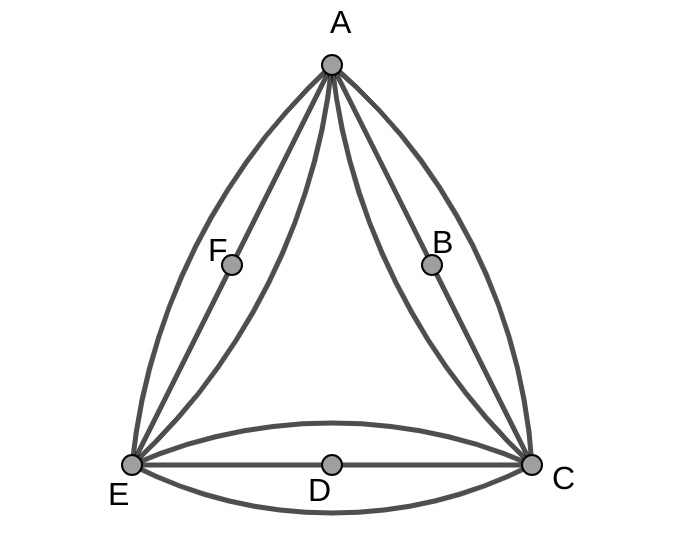
\includegraphics[width=70mm]{parallel}
  \caption{Simplicity is necessary}
  \label{fig:parallel}
\end{figure}

\begin{remark}
  Allowing triangulated disks (i.e. planar graphs with at most one face greater
  than $3$), the conjecture does not hold. For example, the graph on figure
  \ref{fig:sungraph} does not have a $2$-coupon coloring from similar reasons as
  the previous one. We will show later that this graph is a member of a bigger
  graph family without $2$ disjoint dominating sets.
\end{remark}

\begin{figure}[ht]
  \centering
  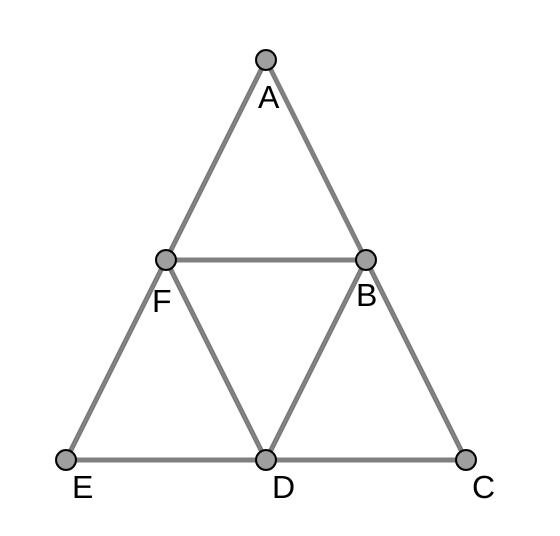
\includegraphics[width=70mm]{sungraph}
  \caption{The conjecture does not hold for triangulated disks}
  \label{fig:sungraph}
\end{figure}

There are some sufficient conditions known for having a total domatic number of
at least $2$. We will cover some of them along the way.
The first example is a graph family for which an easy induction shows that they
are $2$-coupon colorable.

\begin{definition}
  A graph is called a stacked graph if it can be constructed from a triangle by
  repeatedly putting a new vertex in a face and connecting it with the vertices on
  the boundary of that face.
\end{definition}
\begin{remark}
  Stacked graphs are triangulated.
\end{remark}
\begin{claim}
  Stacked graphs with at least $4$ vertices are $2$-coupon colorable.
\end{claim}
\begin{proof}
  We can determine the colors of the vertices as the graph is constructed. The
  current coloring will maintain two following two properties.
  \begin{enumerate}
    \item It is a $2$-coupon coloring of the current graph.
    \item Every face has vertices from both color classes.
  \end{enumerate}
  The construction of the graph starts with a simple triangle. Color two vertices
  of the triangle to blue, and the remaining vertex to red. Color the vertex added
  to the graph in the first step to red. This coloring has the desired properties.
  When a vertex is inserted into a face, color the new vertex to red, if there is
  only one red vertex on the face's boundary, and blue otherwise. This trivially
  maintains the desired properties.
\end{proof}

\section{Outerplanar and triangulated Hamiltonian graphs}
Zoltán Lóránt Nagy showed that the conjecture of Goddard and Henning holds for
Hamiltonian graphs. For this, he characterized the $2$-coupon colorable
maximal outerplanar graphs.

\begin{definition}
   A graph is outerplanar if it has a planar drawing for which all vertices
   belong to the outer face. A maximal outerplanar graph is an outerplanar graph
   such that adding any edge results in a not outerplanar graphs.
\end{definition}
\begin{remark}
  Te outer face of a maximal outerplanar graph is a Hamiltonian cycle.
\end{remark}

In order to provide the mentioned characterization we need to introduce a few
notions first.
\begin{definition}
  Let $G$ be a maximal outerplanar graph of order $n \ge 3$. The $M(G)$ sun graph
  of $G$ is obtained by gluing a triangle to each edge of the outer face.
\end{definition}
\begin{remark}
  $M(G)$ is a maximal outerplanar graph with $2n$ vertices, from which $n$ has
  degree $2$. The graph on figure $\ref{fig:sungraph}$ is the sun graph of
  the $BDE$ triangle.
\end{remark}
\begin{definition}
  A vertex $v$ of a maximal outerplanar graph is called a central vertex if the
  following $3$ conditions hold.
  \begin{enumerate}
    \item $deg(v) \ge 3$
    \item Every neighbor of $v$ has degree at least $3$
    \item For every $u, w$ neighbors of $v$ the length of the $uw$ path on the
    outer face not containing $v$ is divisible by $4$.
  \end{enumerate}
\end{definition}
\begin{claim}
  The outer face of a maximal outerplanar graph does not contain two consecutive
  central vertices.
\end{claim}
\begin{proof}
  Suppose there exists an $uv$ edge on the outer face such that $u$ and $v$ are
  central vertices. Because of the maximality of the graph there exists a $uvw$
  triangle. Index the vertices along the outer face form $v = v_1$ to $u = v_{n}$.
  Suppose $w = v_i$. From the centrality of $v$ follows that $i \equiv 2\
  (\textrm{mod}\ 4)$. On the other hand $u$ is also a central vertex, hence
  $i \equiv 1\ (\textrm{mod}\ 4)$.
\end{proof}
\begin{definition}
  A generalized sun graph is a maximal outerplanar graph of order
  $n \equiv 2\ (\textrm{mod}\ 4)$ such that the number of
  degree $2$ vertices plus the number of central vertices is $n/2$.
\end{definition}
\begin{remark}
  Every second vertex of the outer face in a generalized sun graph is either
  central or has degree $2$.
\end{remark}

The key characterization theorem is the following.

\begin{thm}\label{thm:outerplanar}
  Let $G$ be a maximal outerplanar graph. $G$ admits $2$ disjoint total dominating
  sets if and only if $G$ is not a generalized sun graph.
\end{thm}

For proving this theorem we need some observations about generalized sun graphs.

\begin{proof}[Proof of Theorem \ref{thm:outerplanar}]
  First we show that generalized sun graphs do not have $2$ disjoint total
  dominating sets. The proof goes by induction on the $n = 4k + 2$ number of vertices.
  For $k = 1$ there is only one generalized sun graph and it does not admit $2$
  disjoint total dominating sets. (Shown on figure \ref{fig:sungraph}.)
  Suppose $k \ge 2$ and $G$ is a generalized sun graph of order $4k + 2$. Index
  the vertices along the outer face from $v_1$ to $v_{4k + 2}$, such that every
  vertex with an odd index is central or has degree $2$. Let $c$ be a $2$-coloring of
  the graph. We show that $c$ cannot be a $2$-coupon coloring. The cardinality of the
  vertices implies that there must be two consecutive vertices $v_{2i}$ and $v_{2i + 2}$
  with the same color (say white). If $v_{2i}$ has only white neighbors, then this
  coloring is not a $2$-coupon coloring. So suppose $v_{2i}$ has a black neighbor
  $v_j$. In this case, $v_{2i}$ is a central vertex. The $v_{2i}v_j$ edge cuts the graph
  into two parts ($v_{2i}v_j$ is an edge in both graphs). Both of
  these graphs are generalized sun graphs, as $v_{2i}$ either remains a central
  vertex or become a vertex of degree $2$ in these smaller graphs, whereas other
  central vertices remain central vertices. By induction, the restriction of
  $c$ is not a $2$-coupon coloring in either of the smaller graphs. If there is
  a vertex $v_l$ with a monochromatic neighborhood in one of the smaller graphs
  and $l \neq 2i, l \neq j$, then $v_l$ has the same neighborhood in $G$, hence
  all its neighbors are from the same color class. $v_{2i}$ cannot violate the
  condition, as it was chosen in a way that it has both a black and a white neighbor
  in both graphs. Thus the only remaining case is when $v_j$ has a monochromatic
  neighborhood in both graphs. But in this case, all of its neighbors are from
  the same color class as $v_{2i}$, so it has a monochromatic neighborhood also
  in $G$.
\end{proof}

\begin{remark}
  With a slight modification of the proof it can be shown that the vertices of a
  generalized sun graph cannot be colored in a way that every degree $2$ or central
  vertex has neighbors from both color classes.
\end{remark}

\begin{lemma}
  The outer face of a maximal outerplanar graph has a chord ...
\end{lemma}

\begin{thm}
  Every triangulated graph with a Hamiltonian circle admits $2$ disjoint
  dominating sets.
\end{thm}
\begin{proof}
  Let $G$ be a triangulated Hamiltonian graph and let $n$ denote the number of
  vertices in $G$.

  If $n \equiv 0\ (\textrm{mod}\ 4)$, then it is easy to find a $2$-coupon coloring:
  color the vertices along the boundary of the outer face by repeating the pattern
  $BBWW$.

  If $n \equiv 1\ (\textrm{mod}\ 4)$, then the same coloring method almost works.
  There is only $1$ vertex that has $2$ black neighbors on the outer face.
\end{proof}


(Hypergraph connection ???)


\chapter{Restricted 2-factors}
\section{Connection}

\begin{thm}
  Let $G$ be a triangulated planar graph. If all the vertices of $G$ have an
  odd degree, then there exists a coupon coloring with $2$ colors.
\end{thm}
\begin{proof}
  ...
\end{proof}

\section{Barnette's conjecture}

\begin{conj}
  Every 3-connected cubic planar bipartite graph is Hamiltonian.
\end{conj}


\end{document}
